% ============================================================
%  PROBLEM 3 — worked example
%  Shows: the \newfloat "Algorithm" environment declared in main.tex,
%         a matrix, a case distinction and a full-width figure.
% ============================================================

\section*{Problem 3}
\phantomsection
\addcontentsline{toc}{section}{Problem 3}

The task is to find the roots of a polynomial in the complex plane by
iteration, and to determine which starting points converge to which root. The
polynomial is

\begin{equation} \label{poly}
	p(z) = z^3 - 1 \; \; \; \text{, } z \in \mathbb{C}
\end{equation}

The three roots of \cref{poly} are known exactly — they are the cube roots of
unity, evenly spaced on the unit circle:

\begin{equation} \label{roots}
	z_k = e^{2\pi i k/3} \; \; \; \text{, } k = 0, 1, 2
	\; \; \Rightarrow \; \;
	z_0 = 1, \; \; z_{1,2} = -\frac{1}{2} \pm i\frac{\sqrt{3}}{2}
\end{equation}

so the interesting question is not where the roots are but how an iterative
method finds them. Newton's method applied to \cref{poly} generates the
sequence

\begin{equation} \label{newton}
	z_{n+1} = z_n - \frac{p(z_n)}{p'(z_n)}
	= z_n - \frac{z_n^3 - 1}{3z_n^2}
	= \frac{2z_n^3 + 1}{3z_n^2}
\end{equation}

The iteration of \cref{newton} is undefined at $z_n = 0$, where the derivative
vanishes; in practice that single point is handled by the guard in
\cref{alg:newton}. Read as a map on $\mathbb{R}^2$ rather than on $\mathbb{C}$,
the same step uses the Jacobian of the real and imaginary parts,

\begin{equation} \label{jacobian}
	J =
	\begin{bmatrix}
		\dfrac{\partial u}{\partial x} & \dfrac{\partial u}{\partial y} \\[10pt]
		\dfrac{\partial v}{\partial x} & \dfrac{\partial v}{\partial y}
	\end{bmatrix}
	=
	\begin{bmatrix}
		\phantom{-}3(x^2 - y^2) & -6xy \\[4pt]
		\phantom{-}6xy          & \phantom{-}3(x^2-y^2)
	\end{bmatrix}
\end{equation}

whose structure — equal diagonal entries, equal and opposite off-diagonal
entries — is just the Cauchy–Riemann conditions written out, confirming that
the two formulations agree.

Convergence is decided by a tolerance test on successive iterates:

\begin{equation} \label{stop}
	\text{stop when} \; \; \;
	\begin{cases}
		|z_{n+1} - z_n| < \varepsilon & \text{converged, assign to the nearest root of \cref{roots}} \\[4pt]
		n = N_{\max}                  & \text{no convergence, leave the point unassigned}
	\end{cases}
\end{equation}

Newton's method converges quadratically once it is close enough to a simple
root \cite{numrecipes}, so $\varepsilon = 10^{-8}$ and $N_{\max} = 50$ are
generous settings: points that converge at all typically do so within a dozen
iterations. The whole procedure is collected in \cref{alg:newton}.

\begin{algorithm}[htbp]
	\caption{Newton iteration on a grid of starting points. The step is
	\cref{newton} and the stopping rule is \cref{stop}. Written as a generic
	fixed-point loop so it can be reused for any $p(z)$ by changing one line.}
	\label{alg:newton}
	\begin{enumerate}
		\itemsep2pt
		\item Choose a grid of starting points $z^{(0)}$ covering the region of interest.
		\item For each starting point, repeat at most $N_{\max}$ times:
		\begin{enumerate}
			\item If $|p'(z_n)| < \delta$, mark the point as unassigned and stop.
			\item Take the step $z_{n+1} \leftarrow z_n - p(z_n)/p'(z_n)$.
			\item If $|z_{n+1} - z_n| < \varepsilon$, stop: the iteration has converged.
		\end{enumerate}
		\item Assign the converged point to whichever root of \cref{roots} it is nearest.
		\item Colour the starting point by that root, and shade it by the iteration count.
	\end{enumerate}
\end{algorithm}

Colouring every starting point by the root it reaches produces
\cref{fig:newton}. The result is not the three tidy wedges one might expect.
Each root's basin of attraction is an open set with a fractal boundary, and
every boundary point is on the boundary of \emph{all three} basins at once —
so arbitrarily small changes in the starting point can change which root the
method finds. The label of \cref{alg:newton} is deliberately generic: the same
loop, with \cref{newton} swapped for another map, is what Problem 5 refers to
as the general structure.

\begin{figure}[htbp]
	\centering
	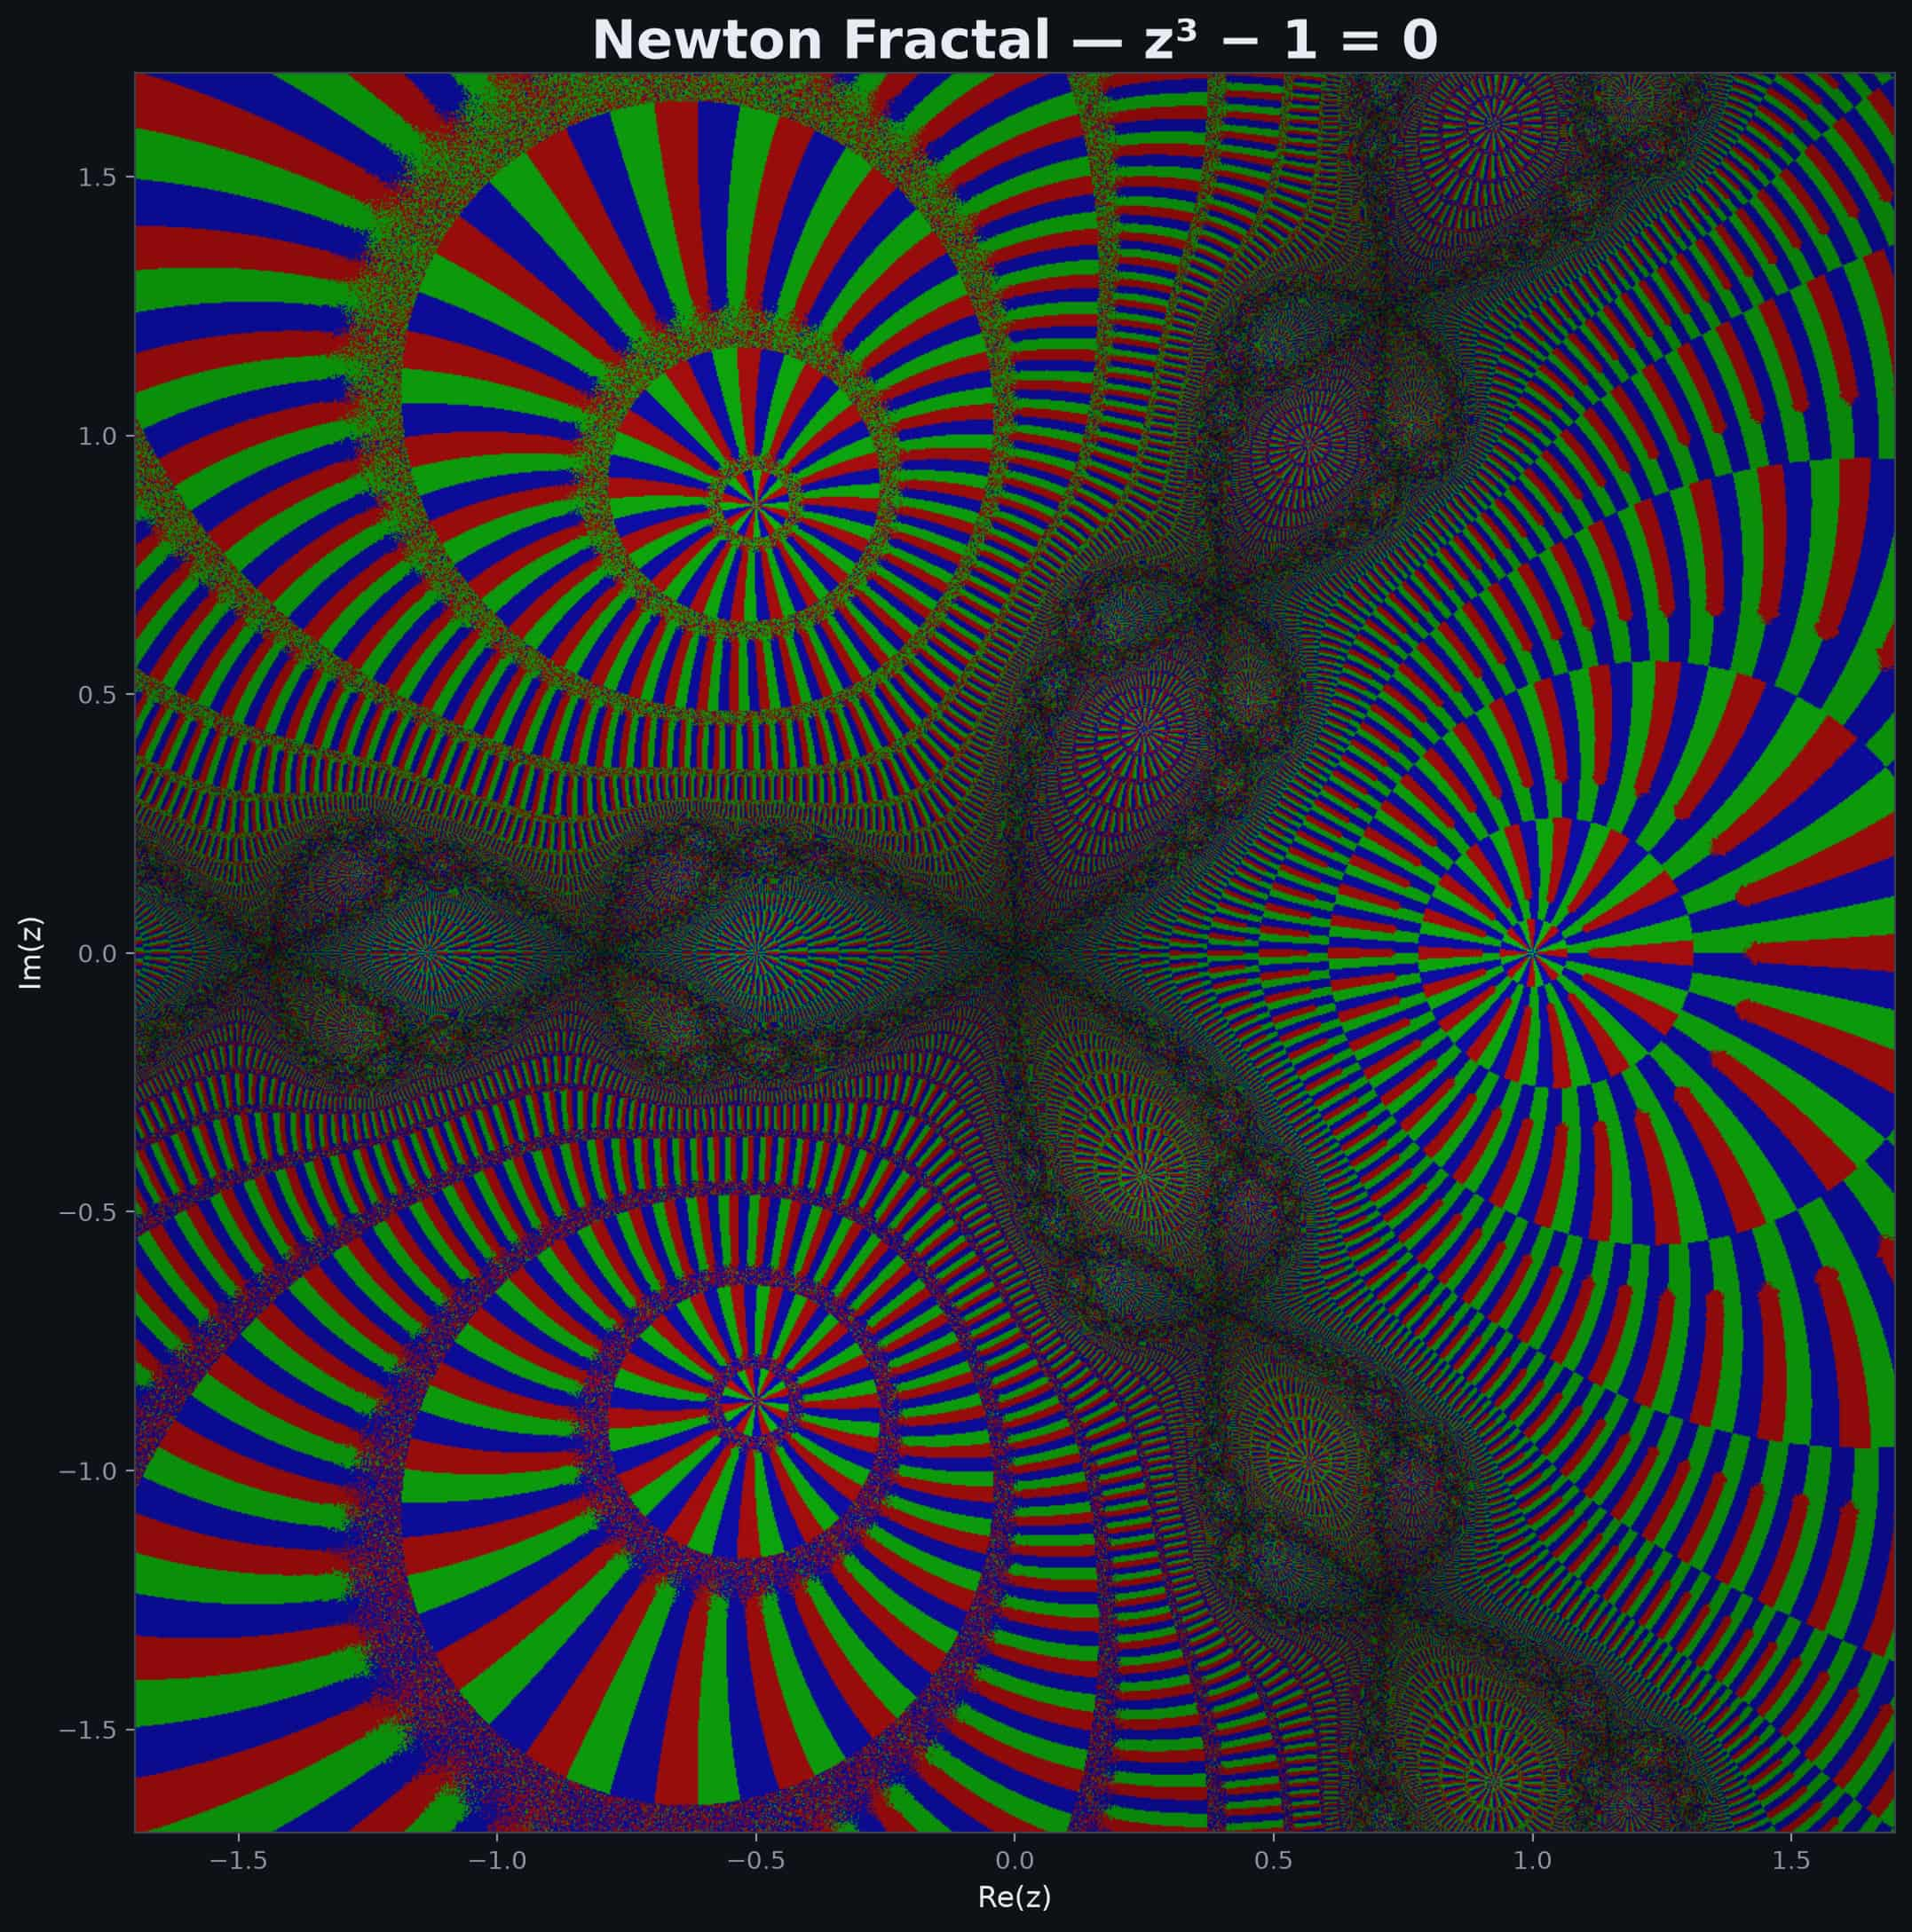
\includegraphics[width=0.85\linewidth]{graphs/newton_fractal}
	\caption{Basins of attraction for \cref{newton} on the square
	$\mathrm{Re}(z), \mathrm{Im}(z) \in [-1.75, 1.75]$. Each colour is one root
	of \cref{roots}; brightness encodes how many iterations \cref{stop} needed.
	The three bright centres are the roots themselves.}
	\label{fig:newton}
\end{figure}

\FloatBarrier
\newpage
